\subsubsection{UC13 - Elenco funzioni}
\begin{figure}[H]
	\centering
	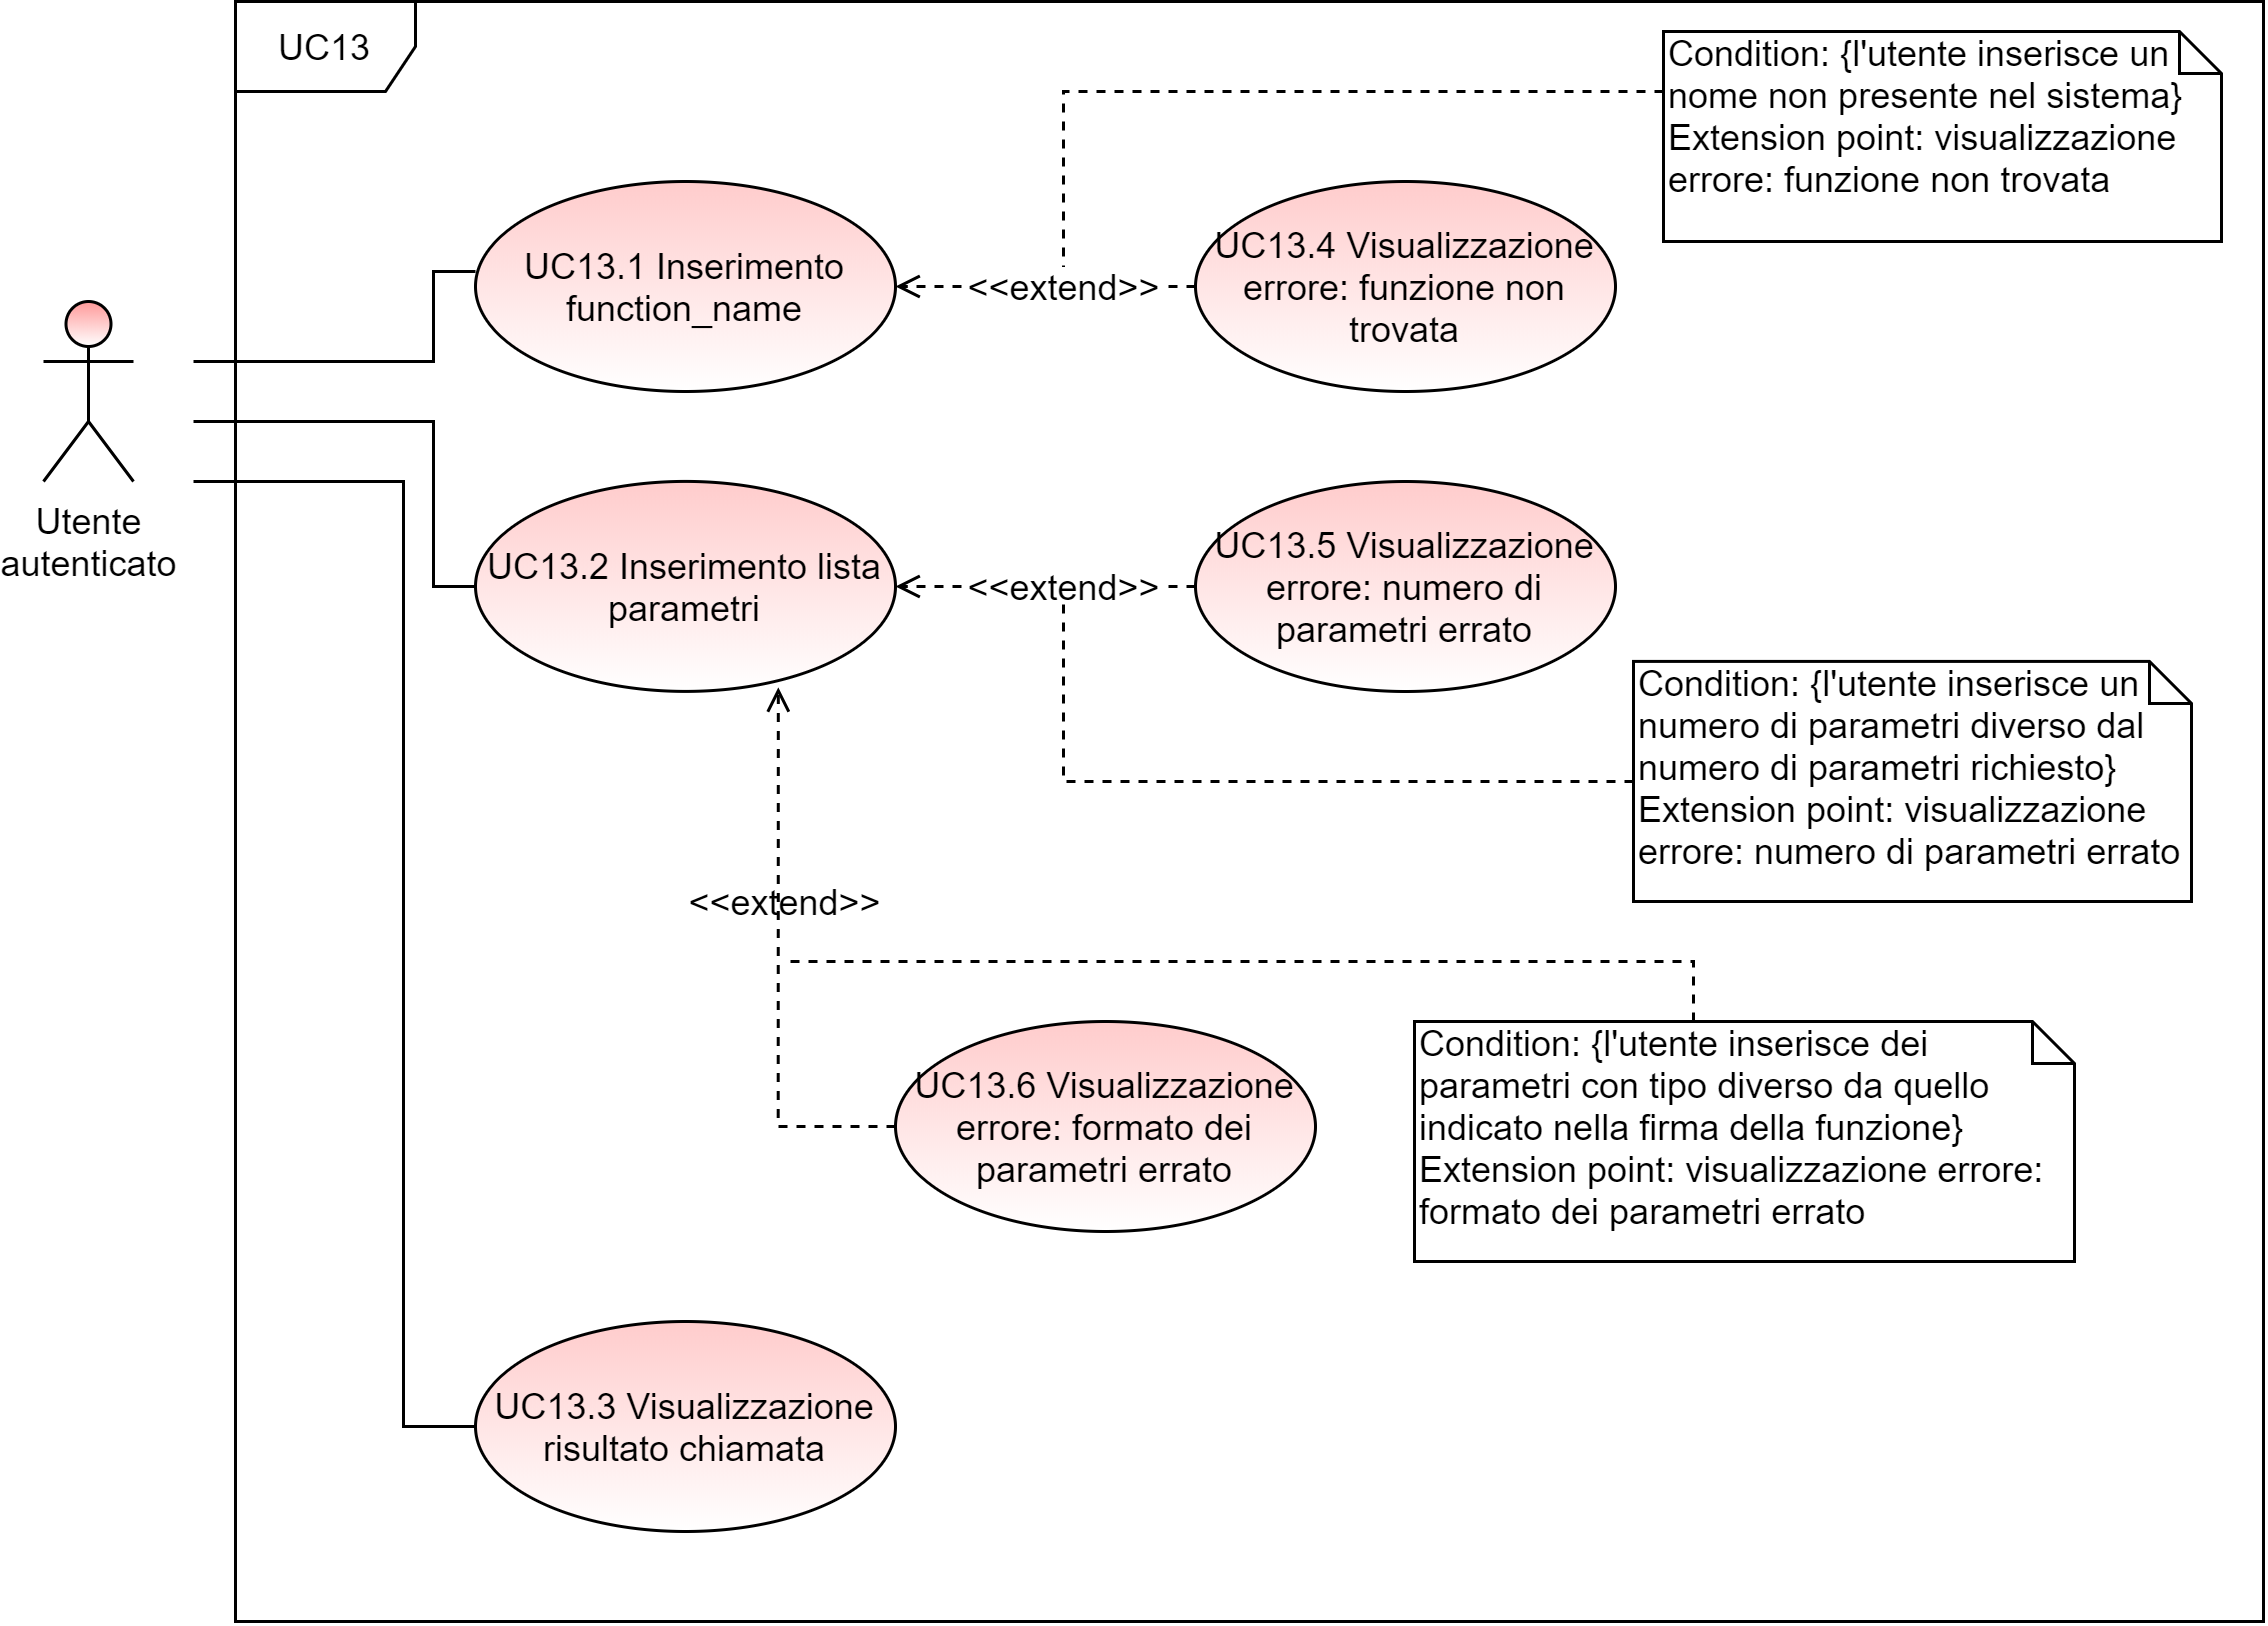
\includegraphics[scale=\ucs]{./res/img/UC13.png}
	\caption {UC13 - Elenco funzioni}
\end{figure}
\begin{itemize}
	\item \textbf{Attori primari:} \ua{};
	\item \textbf{Attori secondari:} \re{};
	\item \textbf{Descrizione:} l’utente richiede la visualizzazione della lista di tutte le funzioni disponibili presso il servizio oppure della lista delle funzioni di sua proprietà. Il sistema stampa a video tale lista;
	\item \textbf{Scenario principale:} 
	\begin{itemize}
		\item l'utente inserisce correttamente ed esegue il comando \lista{} oppure il comando \plista{};
		\item viene visualizzata la lista completa di tutte le funzioni disponibili oppure soltanto di quelle di proprietà dell’utente. 
	\end{itemize}
	\item \textbf{Precondizione:} l’utente desidera visualizzare la lista di tutte le funzioni oppure la lista delle funzioni di sua proprietà;
	\item \textbf{Postcondizione:} la CLI\ped{\textit{G}} riporta la lista di tutte le funzioni disponibili oppure la lista delle funzioni di proprietà dell’utente.
\end{itemize}